\newpage
\section{Prospetto economico}
In questo paragrafo sono presentate, per ciascun periodo del progetto, le ore di impegno calcolate a preventivo per i ruoli coinvolti, divise tra ore di lavoro e ore contabilizzate.\\
 Si ricorda che il periodo di \ARM\ non è a carico del \termine{committente} e quindi non sarà considerata nel calcolo del preventivo.
 
\subsection{\ARD}
Nel periodo riguardante la fase di \ARD\ le ore tra i ruoli sono state divise nel seguente modo:

\begin{table}[h]
	\begin{center}
		\begin{tabular}{|l|c|c|}
			\hline
			\textbf{Ruolo}	& \textbf{Ore} & \textbf{Costo} \\
			\hline
			\textit{\Pm} &	3	&	90\\
			\hline
			\textit{\Am}	&	3	&	 60	\\
			\hline
			\textit{\An}	&	30	&	 750	\\
			\hline
			\textit{\Ver}	 & 14	&	 210	\\
			\hline
			\textbf{Totale} &	 50	&	1110\\
			\hline
		\end{tabular}
	\end{center}
	\caption{Incidenza ore su costo per ruolo, \ARD}
\end{table}

\begin{figure}[H]
	\centering 
	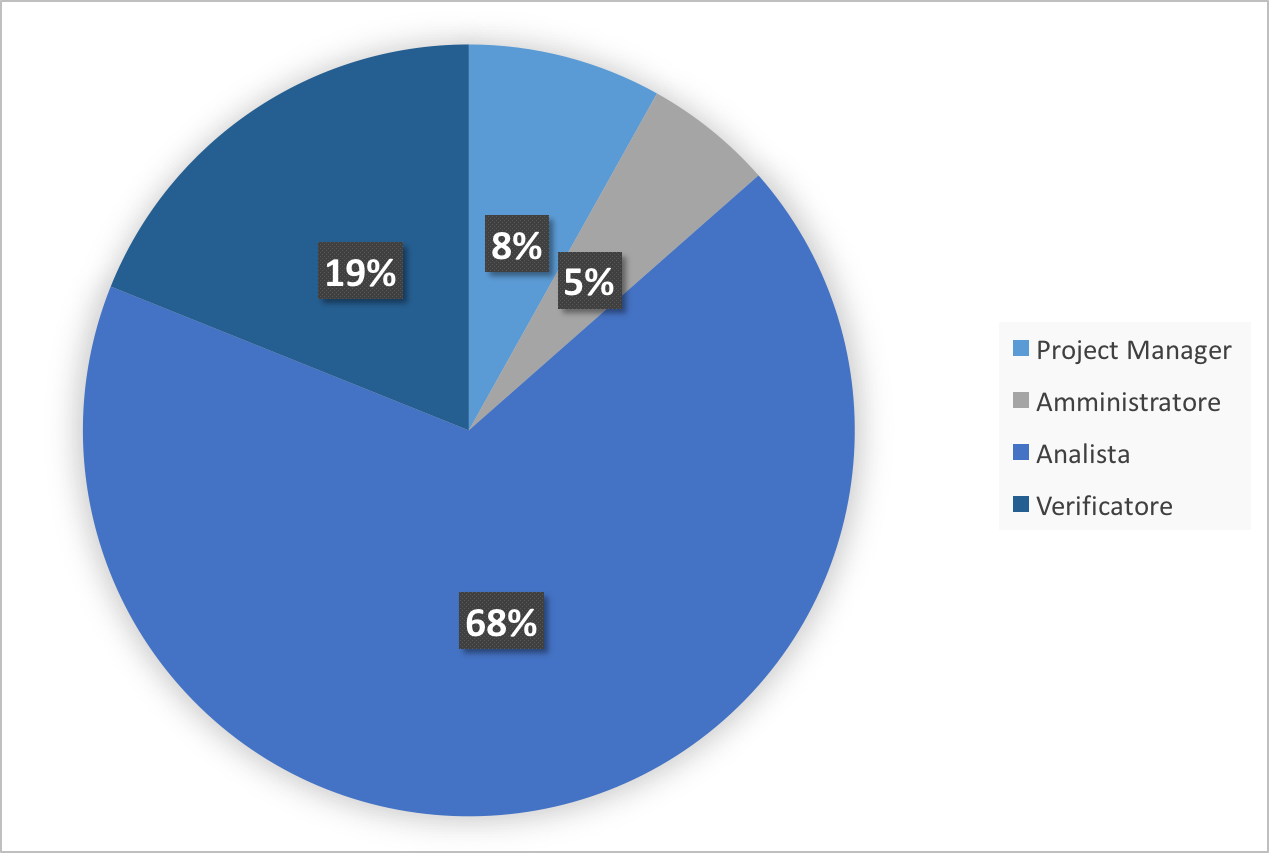
\includegraphics[scale=0.7]{Immagini/GraficiTorteSezione6/ARD.png}
	\caption{Costo per ruolo, \ARD}
\end{figure}

\newpage
\subsection{\PA}
Nel periodo riguardante la \PA\ le ore tra i ruoli sono state divise nel seguente modo:

\begin{table}[h]
	\begin{center}
		\begin{tabular}{|l|c|c|}
			\hline
			\textbf{Ruolo}	& \textbf{Ore} &	\textbf{Costo}	 \\
			\hline
			\textit{\Pm}	&	6	&	180\\
			\hline
			\textit{\Am}	&	7	&	140\\
			\hline
			\textit{\Prog}	&	120	&	2640\\
			\hline
			\textit{\Ver}	&	65	&	975\\
			\hline
			\textbf{Totale}	&	198	&	3935\\
			\hline
		\end{tabular}
	\end{center}
	\caption{Incidenza ore su costo per ruolo, \PA}
\end{table}

\begin{figure}[H]
	\centering 
	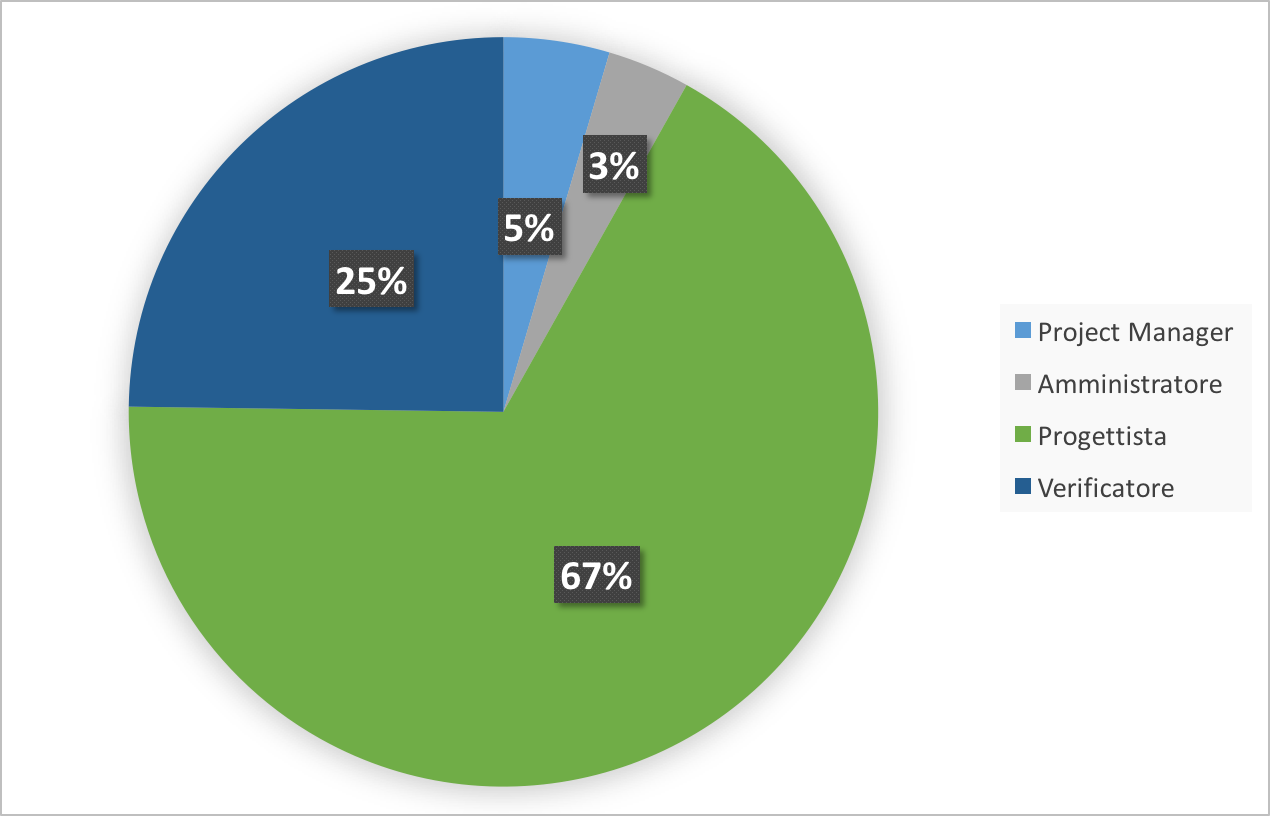
\includegraphics[scale=0.7]{Immagini/GraficiTorteSezione6/PA.png}
	\caption{Costo per ruolo, \PA}
\end{figure}

\newpage
\subsection{\PD}
Nel periodo riguardante la \PD\ le ore tra i ruoli sono state divise nel seguente modo:

\begin{table}[h]
	\begin{center}
		\begin{tabular}{|l|c|c|}
			\hline
			\textbf{Ruolo}	& \textbf{Ore} &	\textbf{Costo}	 \\
			\hline
			\textit{\Pm}	&	7	&	210\\
			\hline
			\textit{\Am}	&	7	&	140\\
			\hline
			\textit{\Prog}	&	65	&	1430\\
			\hline
			\textit{\Ver}	&	42	&	630\\
			\hline
			\textbf{Totale}	&	121	&	2410\\
			\hline
		\end{tabular}
	\end{center}
	\caption{Incidenza ore su costo per ruolo, \PD}
\end{table}

\begin{figure}[H]
	\centering 
	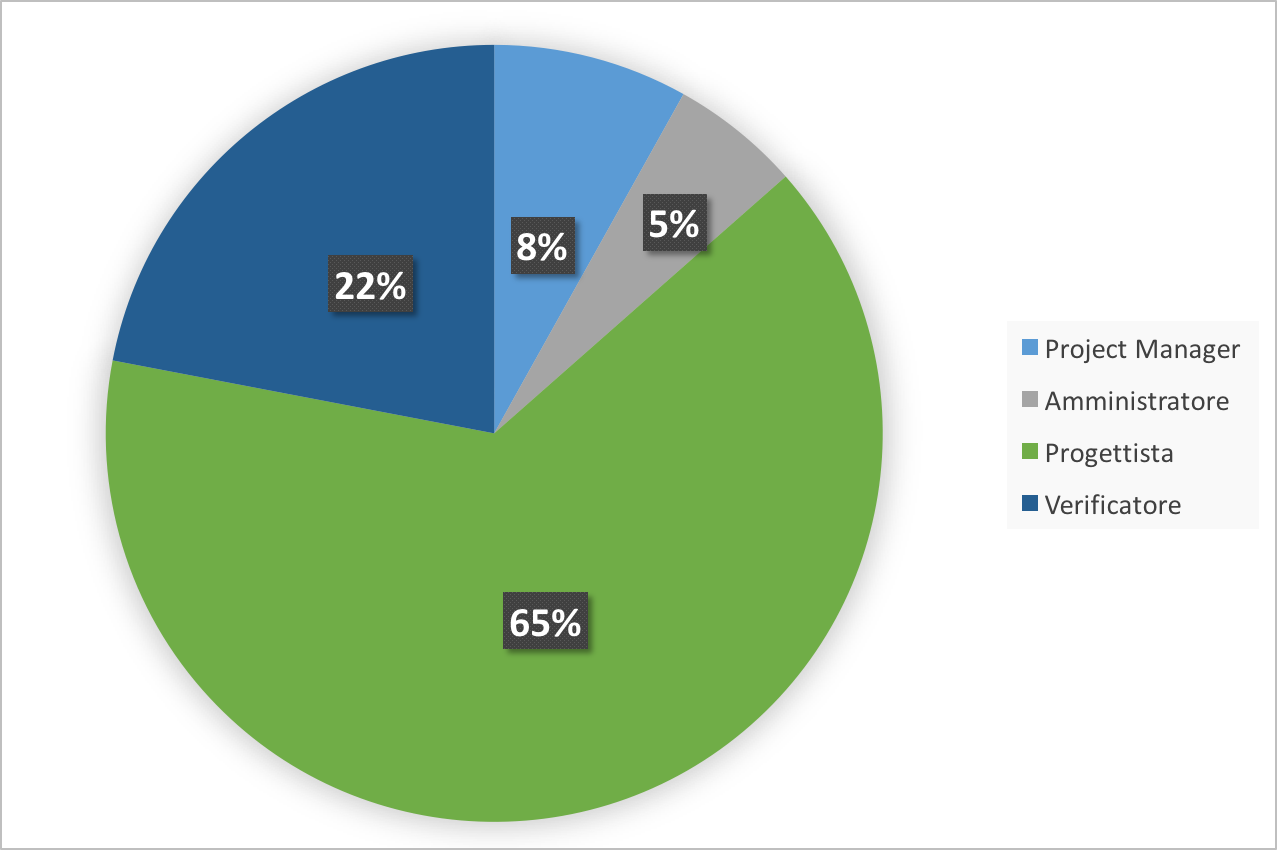
\includegraphics[scale=0.7]{Immagini/GraficiTorteSezione6/PD.png}
	\caption{Costo per ruolo, \PD}
\end{figure}

\newpage
\subsection{\COD}
Nel periodo riguardante la \COD\ le ore tra i ruoli sono state divise nel seguente modo:

\begin{table}[h]
	\begin{center}
		\begin{tabular}{|l|c|c|}
			\hline
			\textbf{Ruolo}	& \textbf{Ore} &	\textbf{Costo}	 \\
			\hline
			\textit{\Pm}	&	11	&	330\\
			\hline
			\textit{\Am}	&	6	&	120	\\
			\hline
			\textit{\Prog}	&	21	&	462	\\
			\hline
			\textit{\Progr}	&	137	&	2055\\
			\hline
			\textit{\Ver}	&	77	&	1155\\
			\hline
			\textbf{Totale}	&	252	&	4122\\
			\hline
		\end{tabular}
	\end{center}
	\caption{Incidenza ore su costo per ruolo, \COD}
\end{table}

\begin{figure}[H]
	\centering 
	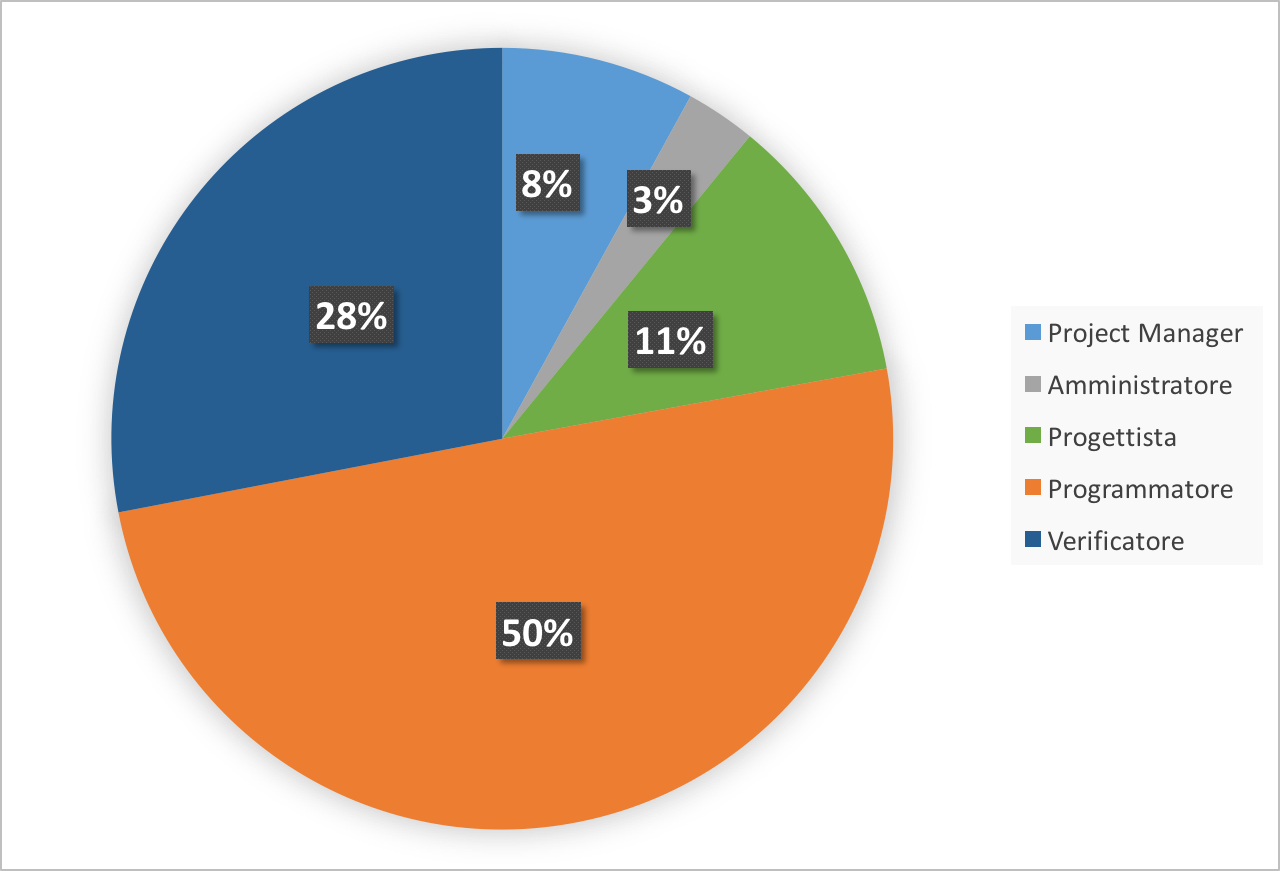
\includegraphics[scale=0.7]{Immagini/GraficiTorteSezione6/COD.png}
	\caption{Costo per ruolo, \COD}
\end{figure}

\newpage
\subsection{\VV}
Nel periodo riguardante la \VV\ le ore tra i ruoli sono state divise nel seguente modo:

\begin{table}[h]
	\begin{center}
		\begin{tabular}{|l|c|c|}
			\hline
			\textbf{Ruolo}	& \textbf{Ore} &	\textbf{Costo}	 \\
			\hline
			\textit{\Pm}	&	14	&	420		\\
			\hline
			\textit{\Am}	&	8	&	160		\\
			\hline
			\textit{\Prog}	&	12	&	264	\\
			\hline
			\textit{\Progr}	&	11	&	165	\\
			\hline
			\textit{\Ver}	&	69	&	1035	\\
			\hline
			\textbf{Totale}	&	114	&	2044	\\
			\hline
		\end{tabular}
	\end{center}
	\caption{Incidenza ore su costo per ruolo, \VV}
\end{table}

\begin{figure}[H]
	\centering 
	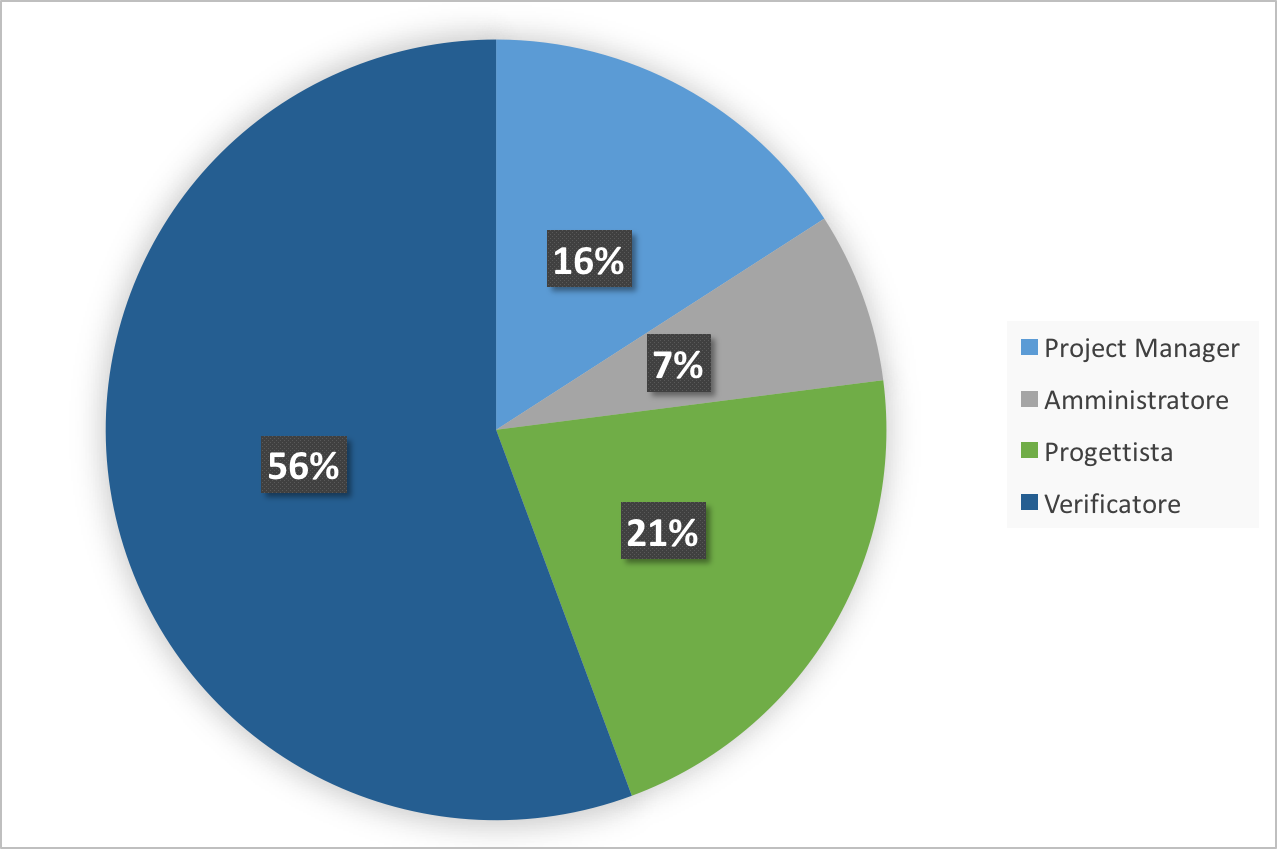
\includegraphics[scale=0.7]{Immagini/GraficiTorteSezione6/VV.png}
	\caption{Costo per ruolo, \VV}
\end{figure}

\newpage
\subsection{Totale}
\subsubsection{Ore totali}
Le ore totali, previste per la realizzazione dell'intero progetto, comprese le ore di investimento, sono riportate nella tabella seguente.

\begin{table}[h]
	\begin{center}
		\begin{tabular}{|l|c|c|c|}
			\hline
			\textbf{Ruolo}	& \textbf{Ore} &	\textbf{Ore remunerabili}	 &\textbf{Costo} \\
			\hline
			\textit{\Pm}	&	61	&	41	&	1230	\\
			\hline
			\textit{\Am}	&	50	&	31	&	620	\\
			\hline
			\textit{\An}	&	105	&	30	&	750	\\
			\hline
			\textit{\Prog}	&	218	&	218	&	4796	\\
			\hline
			\textit{\Progr}	&	148	&	148	&	2220	\\
			\hline
			\textit{\Ver}	&	332	&	267	&	4005	\\
			\hline
			\textbf{Totale}	&	914 & 735 & 13621	\\
			\hline
		\end{tabular}
	\end{center}
	\caption{Costo totale per ruolo}
\end{table}

\begin{figure}[H]
	\centering 
	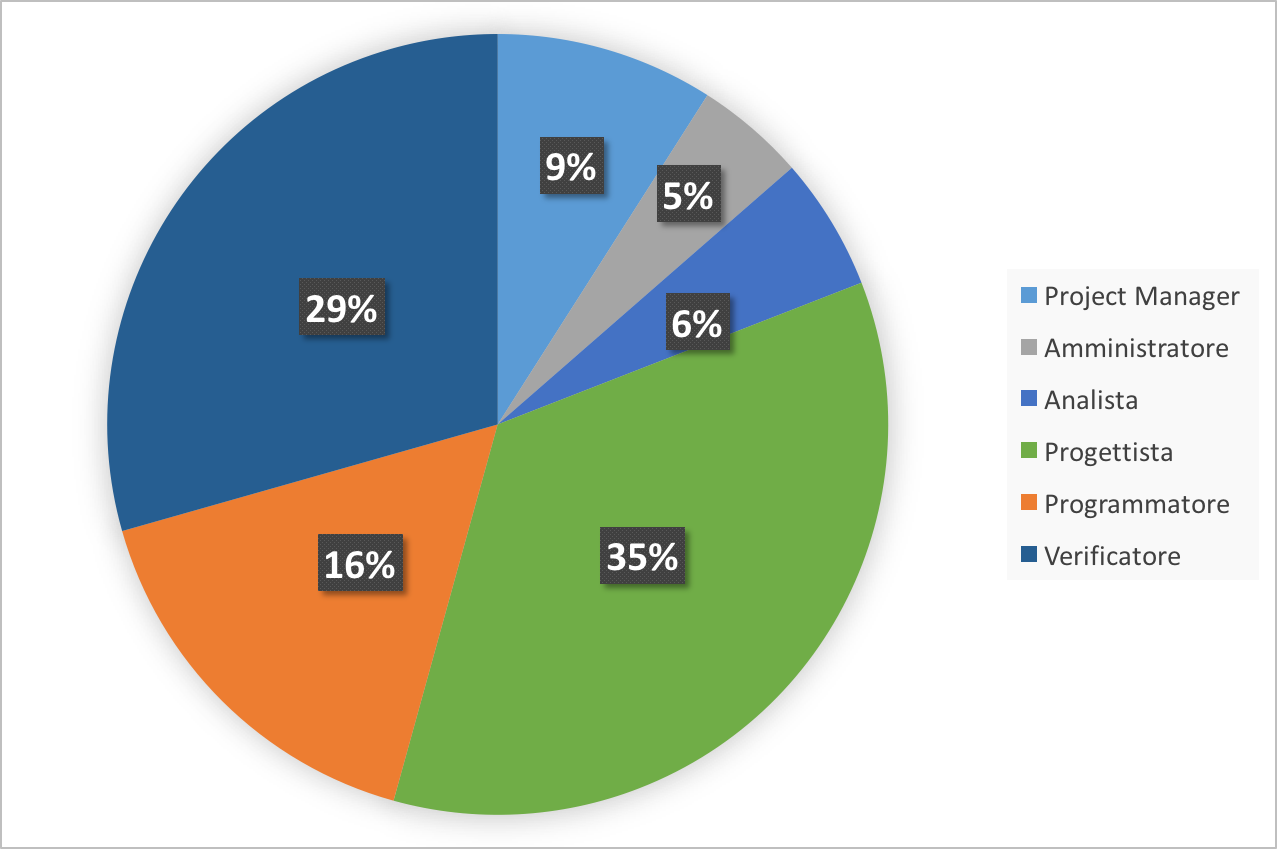
\includegraphics[scale=0.7]{Immagini/GraficiTorteSezione6/TOT.png}
	\caption{Costo totale per ruolo}
\end{figure}

\subsubsection{Conclusioni}
Il costo totale del progetto, indicato nella tabella 20, ammonta a \textbf{\euro 13621} rispettando il primo impegno preso al momento della gara per aggiudicarsi il capitolato.\\